\documentclass[12pt]{article}

\usepackage[utf8]{inputenc}
\usepackage[T1]{fontenc}
\usepackage[polish,provide=*]{babel}
\usepackage{lmodern}
\usepackage{amsmath}
\usepackage{latexsym,amsfonts,amssymb,amsthm,amsmath}
\usepackage{enumitem}
\usepackage{float}
\usepackage{hyperref}
\usepackage{graphicx}
\usepackage{subcaption}
\usepackage{booktabs}
\graphicspath{{./images/}}

\setlength{\parindent}{0in}
\setlength{\oddsidemargin}{0in}
\setlength{\textwidth}{6.5in}
\setlength{\textheight}{8.8in}
\setlength{\topmargin}{0in}
\setlength{\headheight}{18pt}

\title{Ciało Doskonale Czarne}
\author{Kacper Kłos}

\begin{document}

\maketitle

Abstract

\newpage
\section{Wstęp}
W tym artykule zbadamy zależności opisujące transfer energi między dwoma ciałami za pośrednictwem promieniowania. Wpierw skorzystamy z kostki Lesliego z dostosowywalną temperaturą oraz detektorem promieniowania aby zbadać zależność promieniowania od temperatury dla powierzchni o różnych parametrach. Następnie przy użyciu tego samego detektora oraz żarówki sprawdzimy co dzieje się z odbieranym promieniowaniem wraz ze zmianą odległości między żarówką i detektorem przy stałej temperatury żarówki, a także ze zmianą temperatury przy niezmienej oddległości. Finalnie dla pomiarów kostki Lesliego i żarówki sprawdzimy co się dzieje gdy między źródłem promieniowania a detektorem ustawimy szklany ekran.
\section{Podstawy Teoretyczne}
Przedstawiona tutaj wyprowadzenie używanych w doświadczeniu wzorów jest skróconą wersją wyprowadzenia znajdującego się w \cite{skrypt} skupiającą się na wzorach kluczowych dla doświadczenia.
Jedną z podstawowych metod wymiany ciepła między ciałami jest promieniowanie.
Promieniujące ciało można opisać za pomocą 3 stałych:
\begin{itemize}
    \item współczynnik absorbcji A - ułamek promieniowania jaki zostaje wchłonięty po padnięciu na ciało.
    \item współczynnik odbicia R - ułamek promieniowania jaki zostaje odbity po padnięciu na ciało.
    \item współczynnik transmisji T - ułamek promieniowania jaki zostaje przepuszczony przez ciał po padnięciu na nie.
\end{itemize}
Wszystkie stałe muszą sumować się do 1 ($A+R+T = 1$).
Przydatnym uogólnieniem jest ciało doskonale czarne które cechuje $A=1$ w całym zakresie widma promieniowania.

Wzory używane przy mówieniu o promieniowaniu to:
Strumień promieniowania danej długości fali w zależności od temperatury dla ciała doskonale czarnego:
\begin{equation}
    I(T, \lambda) = \frac{2\pi c^2 h}{\lambda^5} \cdot \frac{1}{\exp(\frac{hc}{\lambda k T}) -1}
    \label{eq:emision_spectrum}
\end{equation}
Oraz wynikające z niego prawo Stefana-Boltzmanna będące sumą po wszystkich długościach fal wzoru \ref{eq:emision_spectrum}:
\begin{equation}
    J_{CDC}(T) = \sigma T^4
    \label{eq:boltzman_law}
\end{equation}
Gdzie $\sigma$ jest stałą Stefana-Boltzmanna.

Wzór ten można uogólnić na ciała inne niż doskonale czarne wprowadzając stałą $\epsilon$ definującą zdolność emisyjne ciała, przekształcające wzór \ref{eq:boltzman_law} na:
\begin{equation}
    J(T) = \epsilon \sigma T^4
    \label{eq:boltzman_law_epsilon}
\end{equation}

Korzystając z tych wzorów możemy znaleźć moc jaką będzie wypromieniowywać dana powierzchnia. Jako że ciało emituje promieniowanie przez swoją temperature ale zarazem przyjmuje promieniowania z otoczenia otrzymujemy wzór:
\begin{equation}
    \Delta P = AS \sigma (T^4-T^4_{ot})
    \label{eq:power_loss}
\end{equation}
W którym A - absorbcja, S - pole powierzchni ciała. 

W przypadku ciał punktowych energia będzie izotropowo rozprowadzona na powierzchini sfery co prowadzi nas do wzoru na strumień mocy:
\begin{equation}
    J(r) = \frac{AS \sigma (T^4-T^4_{ot})}{4\pi r^2}
    \label{eq:power_flux}
\end{equation}

\section{Układ Doświadczalny}
Podstawowym narzędziem z jakiego będziemy korzystać jest detektor promieniowania termiczniego (PASCO TD-8553) dla którego zależność mierzonego napięcia od strumienia mocy jaki pada na miernik jest linowa:
\begin{equation}
    U_d = \alpha J_{pad}-\beta
    \label{eq:measurment_device}
\end{equation}
Detektor w pomiarach będzie podłączony do miernika uniwersalnego BRYMEN BM827s do pomiaru napięcia.
\subsection{Kostka Lesliego}
W pierwszej części doświadczenia zbadamy emisyjność różnych powierzchni kostki Lesliego (3B Scientific Physics U8498299-230) przy pomocy statycznego miernika promieniowania (rys. \ref{fig:cube_diagram}. 
\begin{figure}[H]
    \centering
    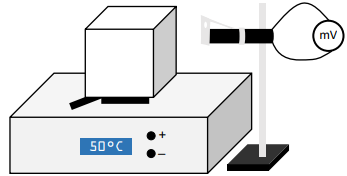
\includegraphics[scale=0.5]{cube}
    \caption{Diagram układu doświadczalnego dla kostki Lesliego (źródło: \cite{skrypt})}
    \label{fig:cube_diagram}
\end{figure}
Kostka składa się z 4 powierzchni: czarnej, białej, metalowej matowej oraz metalowej błyszczącej, do tego kostka może zostać podgrzana od $40 \ ^{\circ}C$ do $120 \ ^{\circ}C$.
Detektor promieniowania kierujemy na kostkę i mierzymy promieniowania dla różnych powierzchni przy zmienianiu temperatury. 
Kluczowe jest zasłanianie detektora osłoną podczas oczekiwania na nagrzanie próbki aby nie nabrał temperatury zakłucającej pomiar.
W trakcie doświadczenia musimy także mierzyć napięcie jakie pokazuje detektor podczas bycia zasłoniętym a żeby móc zidentyfikować jaka część promieniowania pochodzi od ścian a jaka od otoczenia.
Przy najwyższej temperaturze zbadamy co pokarze detektor przy zasłonieniu ścianki czarnej przez szklany ekran.

\subsection{Lampa Stefana-Boltzmana}
W tej części przeprowadzimy walidację prawa Stefana-Boltzmana. Ustawiamy detektor i żarówkę na szynie z zaznaczonymi odległościami (rys. \ref{fig:lamp_diagram}) w celu zmierzenia zależność promieniowania jakie pada na detektor od promieniowania źródła i odległości od niego.

\begin{figure}[H]
    \centering
    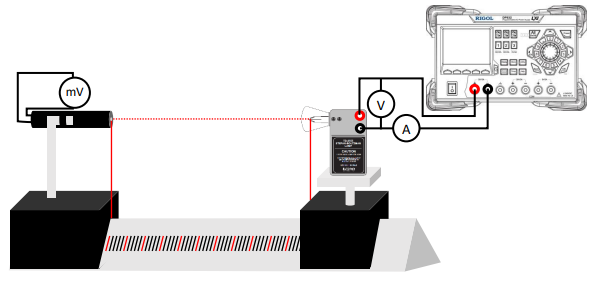
\includegraphics[scale=0.5]{lamp}
    \caption{Diagram układu doświadczalnego dla lampy Stefana-Boltzmana (źródło: \cite{skrypt})}
    \label{fig:lamp_diagram}
\end{figure}

Na początku żarówka i detektor są ustawione blisko siebie żeby zmierzyć zależność strumienia mocy od temperatury.
Zarówkę podłączamy do generatora i mierzymy napięcie oraz natężenia na żarówce za pomocą dwóch mierników BRYMEN BM805s. Zależność temperaturową możemy wyznaczyć wzorami \cite{skrypt}:
\begin{equation}
    T = \frac{R - R_{ref}}{\alpha R_{ref}} + T_{ref}
    \label{eq:temp_bulb}
\end{equation}
We wzorze $T_{ref} = 300\,K$ a $R_{ref} = 0{,}277\, \Omega$, a $\alpha$ opisywane jest zależnością:
\[
    \alpha(K^{-1}) = 0{,}00407 \cdot (\frac{R}{R_{ref}})^{0{,}11778}
\]
Z mierzonych wartości opór otrzymujemy przez prawo ohma:
\[
    R = \frac{U}{I}
\]
Przy pomiarze z najwyższą temperaturą sprawdzamy co się stanie gdy pomiędzy detektor a żarówkę wstawimy szklany ekran.
Po wykonaniu pomiarów zależnych od temperatury, mierzymy zależność od odległości pozostawiając temperaturę stałą poprzez przesówanie detektora na szynie.
\section{Wyniki Pomierów}
We wszystkich pomiarach będziemy korzystać ze zmierzonej stałej temperatury pomieszczenia $T_0 = 22 \, ^{\circ}C$.
Ważne też jest wspomnieć że w poniższej analizie średnią zmiennej $x$ oznaczamy $\bar{x}$, błąd statystyczny $s_x$, błąd pomiarowy $\delta x$ a błąd całkowity $u(x)$.
Wzór na sumaryczny błąd z jakiego będziemy korzystać w momencie kiedy jest kilka punktów pomiarowych to:
\begin{equation}
    u(x) = \sqrt{s_x^2 + (\frac{\delta x}{\sqrt{3}})^2}
    \label{eq:combined_error}
\end{equation}
Gdy pomiar jest pojedyńczy to $u(x) = \delta x$.

Nadmiernie będziemy też korzystać z równania na propagację błędu:
\begin{equation}
    \delta f(x) = \sqrt{\sum_{i} (\frac{df}{dx_i} \delta x_i)^2}
    \label{eq:error_propagation}
\end{equation}

Parę razy wykorzystamy test $\chi^2$ dla którego wzór uogulniony do błędu w x i y przyjmujący formę:
\begin{equation}
    \chi^2 = \sum_{i} \frac{\left( y_i - f(x_i) \right)^2}{\sigma_{y_i}^2 + \left( \frac{df}{dx_i} \cdot \sigma_{x_i} \right)^2}
    \label{eq:chi2}
\end{equation}

\subsection{Kostka Lesliego}
\begin{table}[H]
    \centering
    \begin{tabular}{c|c|cccc|c}
        \toprule
        Nr & $T$ [°C] & $U_b$ [mV] & $U_w$ [mV] & $U_{ms}$ [mV] & $U_{mm}$ [mV] & $U_s$ [mV] \\
        \midrule
        1  & 50  & 2{,}05 & 2{,}05 & 0{,}17 & 0{,}53 & 0{,}15 \\
        2  & 55  & 2{,}56 & 2{,}56 & 0{,}18 & 0{,}63 & 0{,}15 \\
        3  & 60  & 2{,}94 & 2{,}93 & 0{,}23 & 0{,}71 & 0{,}15 \\
        4  & 65  & 3{,}45 & 3{,}41 & 0{,}25 & 0{,}80 & 0{,}17 \\
        5  & 70  & 3{,}89 & 3{,}89 & 0{,}26 & 0{,}95 & 0{,}21 \\
        6  & 75  & 4{,}43 & 4{,}40 & 0{,}29 & 1{,}04 & 0{,}19 \\
        7  & 80  & 4{,}97 & 4{,}94 & 0{,}32 & 1{,}16 & 0{,}17 \\
        8  & 85  & 5{,}43 & 5{,}41 & 0{,}34 & 1{,}28 & 0{,}14 \\
        9  & 90  & 5{,}95 & 5{,}85 & 0{,}38 & 1{,}39 & 0{,}14 \\
        10 & 95  & 6{,}52 & 6{,}48 & 0{,}42 & 1{,}53 & 0{,}17 \\
        11 & 100 & 7{,}12 & 7{,}06 & 0{,}45 & 1{,}71 & 0{,}19 \\
        12 & 105 & 7{,}66 & 7{,}63 & 0{,}50 & 1{,}85 & 0{,}21 \\
        13 & 110 & 8{,}34 & 8{,}32 & 0{,}54 & 2{,}06 & 0{,}24 \\
        14 & 115 & 8{,}87 & 8{,}85 & 0{,}58 & 2{,}15 & 0{,}26 \\
        15 & 120 & 9{,}52 & 9{,}52 & 0{,}63 & 2{,}34 & 0{,}25 \\
        \bottomrule
    \end{tabular}
    \caption{Pomiary napięć dla różnych powierzchni ($U_b$ - czarna, $U_w$ - biała, $U_{ms}$ - metalowa matowa, $U_{mm}$ - metalowa matowa, $U_s$ - tło) w funkcji temperatury $T$.}
    \label{tab:cube_measurements}
\end{table}
Bane uzyskane z badania kostki Lesliego widizmy w tabeli \ref{tab:cube_measurements}, napięcia są mierzone kolejno dla: $U_b$ - strona czarna, $U_w$ - strona biała, $U_{ms}$ - strona metaliczna błyszcząca, $U_{mm}$ - strona metaliczna matowa i $U_s$ - zasłona blokująca promieniowanie.
W tabeli \ref{tab:cube_measurements} widzimy że pomiary dla ściany czarnej i białej są na podobnym poziomie, podczas gdy ściana metalowa błyszcząca ledwo pokazywała wartości większe od promieniowania otoczenia, 
a napięcia wywoływane przez ścianę metalową matową były mniejwięcej stale 4x mniejsze od ściany czarnej, lecz około 3x większe od drugiej metalowej ściany.
Przeanalizujmy dogłębnie dane aby dowiedzieć się więcej o charakterystyce każdej ze ścian.

Wyznaczmy błąd obserwowany podczas badania kostki. Na ekranie kostki Lesligeo widzieliśmy drobne zmianny temperatury dlatego jej błąd uznajemy jako $\delta T = 1 \, ^{\circ}C$.
Podczas gdy błąd z jakim mierzyliśmy napięcie otrzymujemy z instrukcji multimetru \cite{radiation_multimeter} dla naszego zakresu wynosi $\delta U = 0{,}0012 \cdot U + 0{,}02 [mV]$.
Co pozwala nam wyznaczyć błąd dla $U_s$ i jej średnią wartość:
\begin{equation}
    \bar{U_s} = 0{,}186 \, [mV], \quad s_{U_s} = 0{,}039 \, [mV], \quad U_s = 0{,}021 \, [mV], \quad U_s = 0{,}04 \, [mV]
    \label{eq:cube_combined_environment}
\end{equation}
Otrzymaną wartość \eqref{eq:cube_combined_environment} możemy odjąć od każdej ze zmierzonych napięć aby otrzymać jedynie wkład promieniowania pochodzący od kostki otrzymując $U'$ dla każdej ze stron.

Sprawdzmy czy zależność od temperatury zgadza się z z przewidywanym prawa Stefana-Boltzmana \eqref{eq:boltzman_law} poprzez dopasowanie lini do wykresu $U'(T^4)$ dla wszystkich materiałów.

\begin{figure}[H]
    \centering
    \begin{subfigure}{0.45\textwidth}
        \centering
        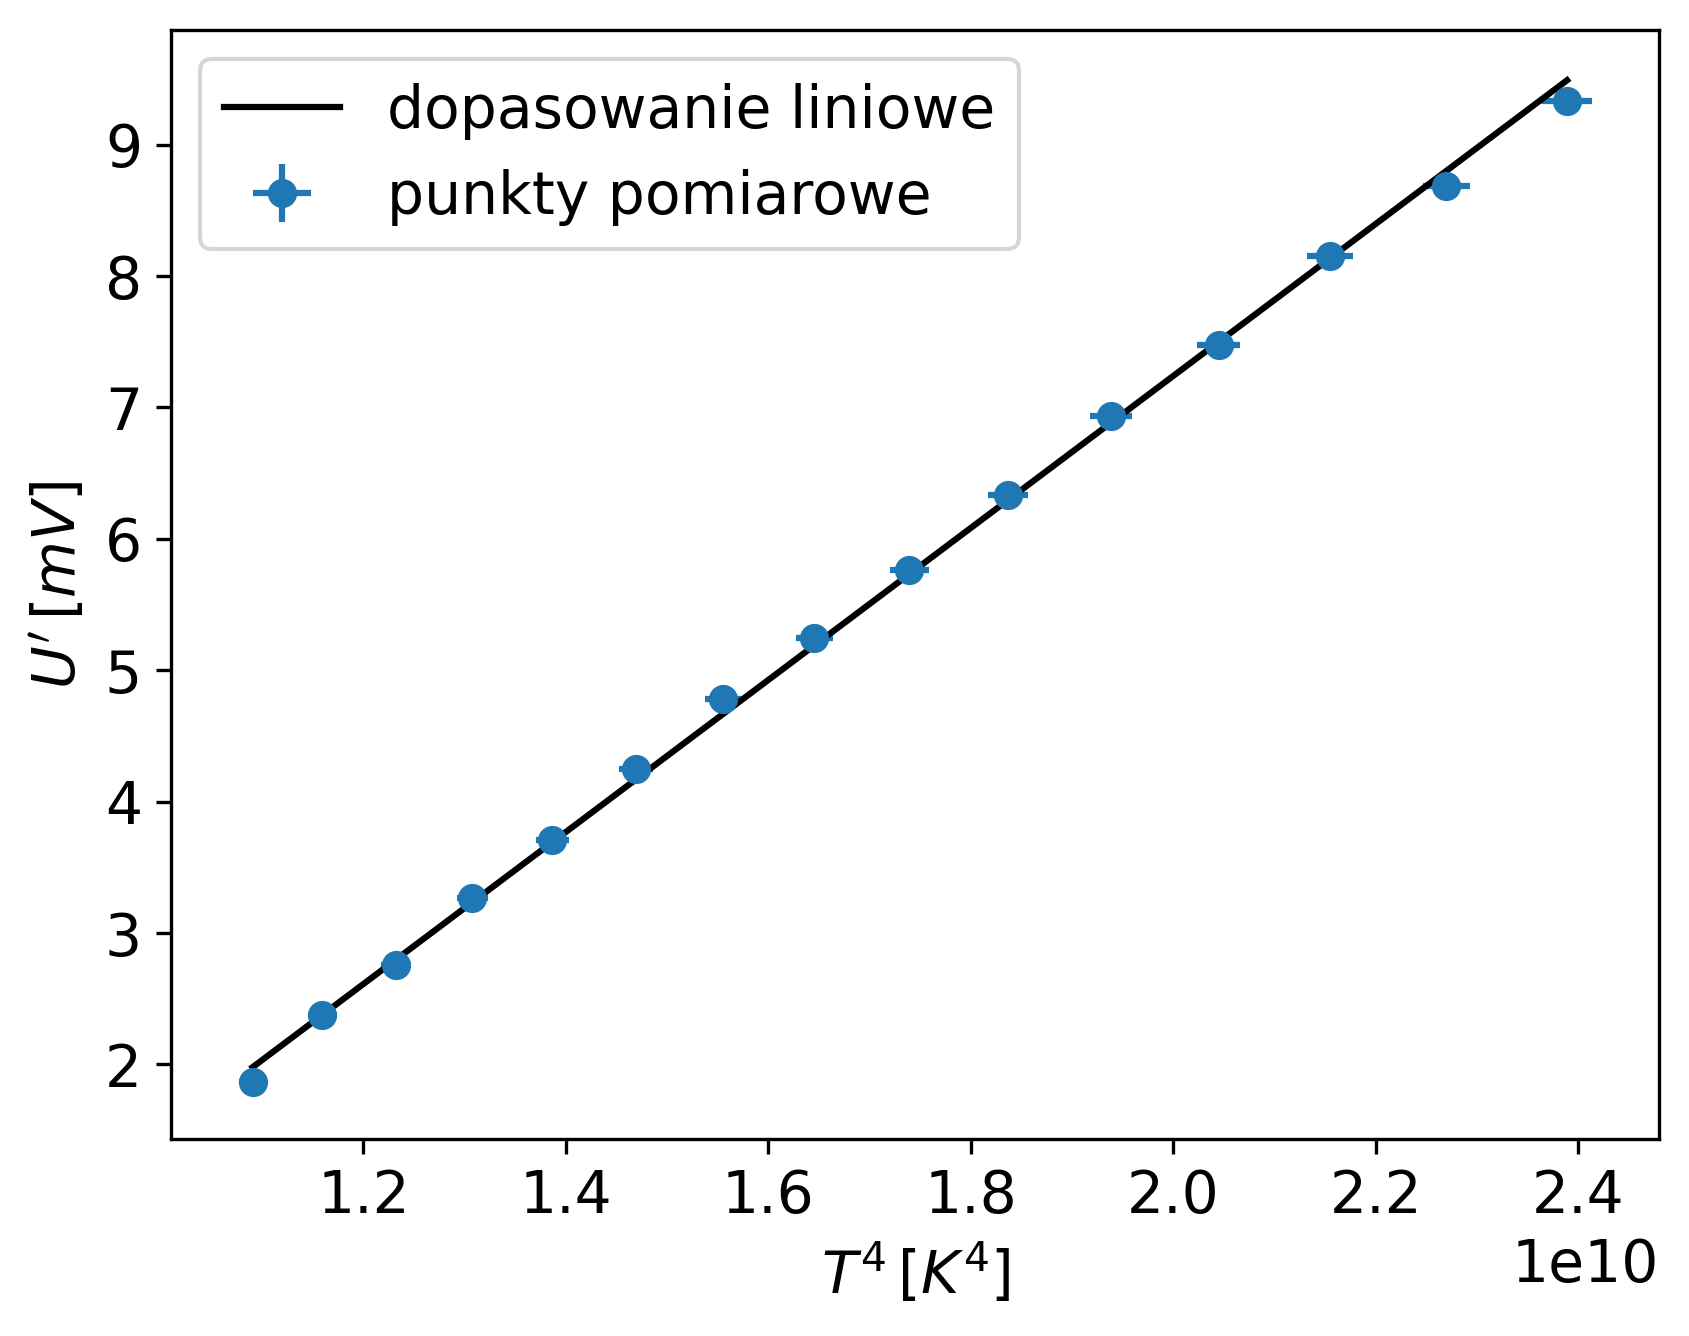
\includegraphics[width=\linewidth]{cube_black}
        \caption{czarna}
        \label{fig:cube_black}
    \end{subfigure}
    \hfill
    \begin{subfigure}{0.45\textwidth}
        \centering
        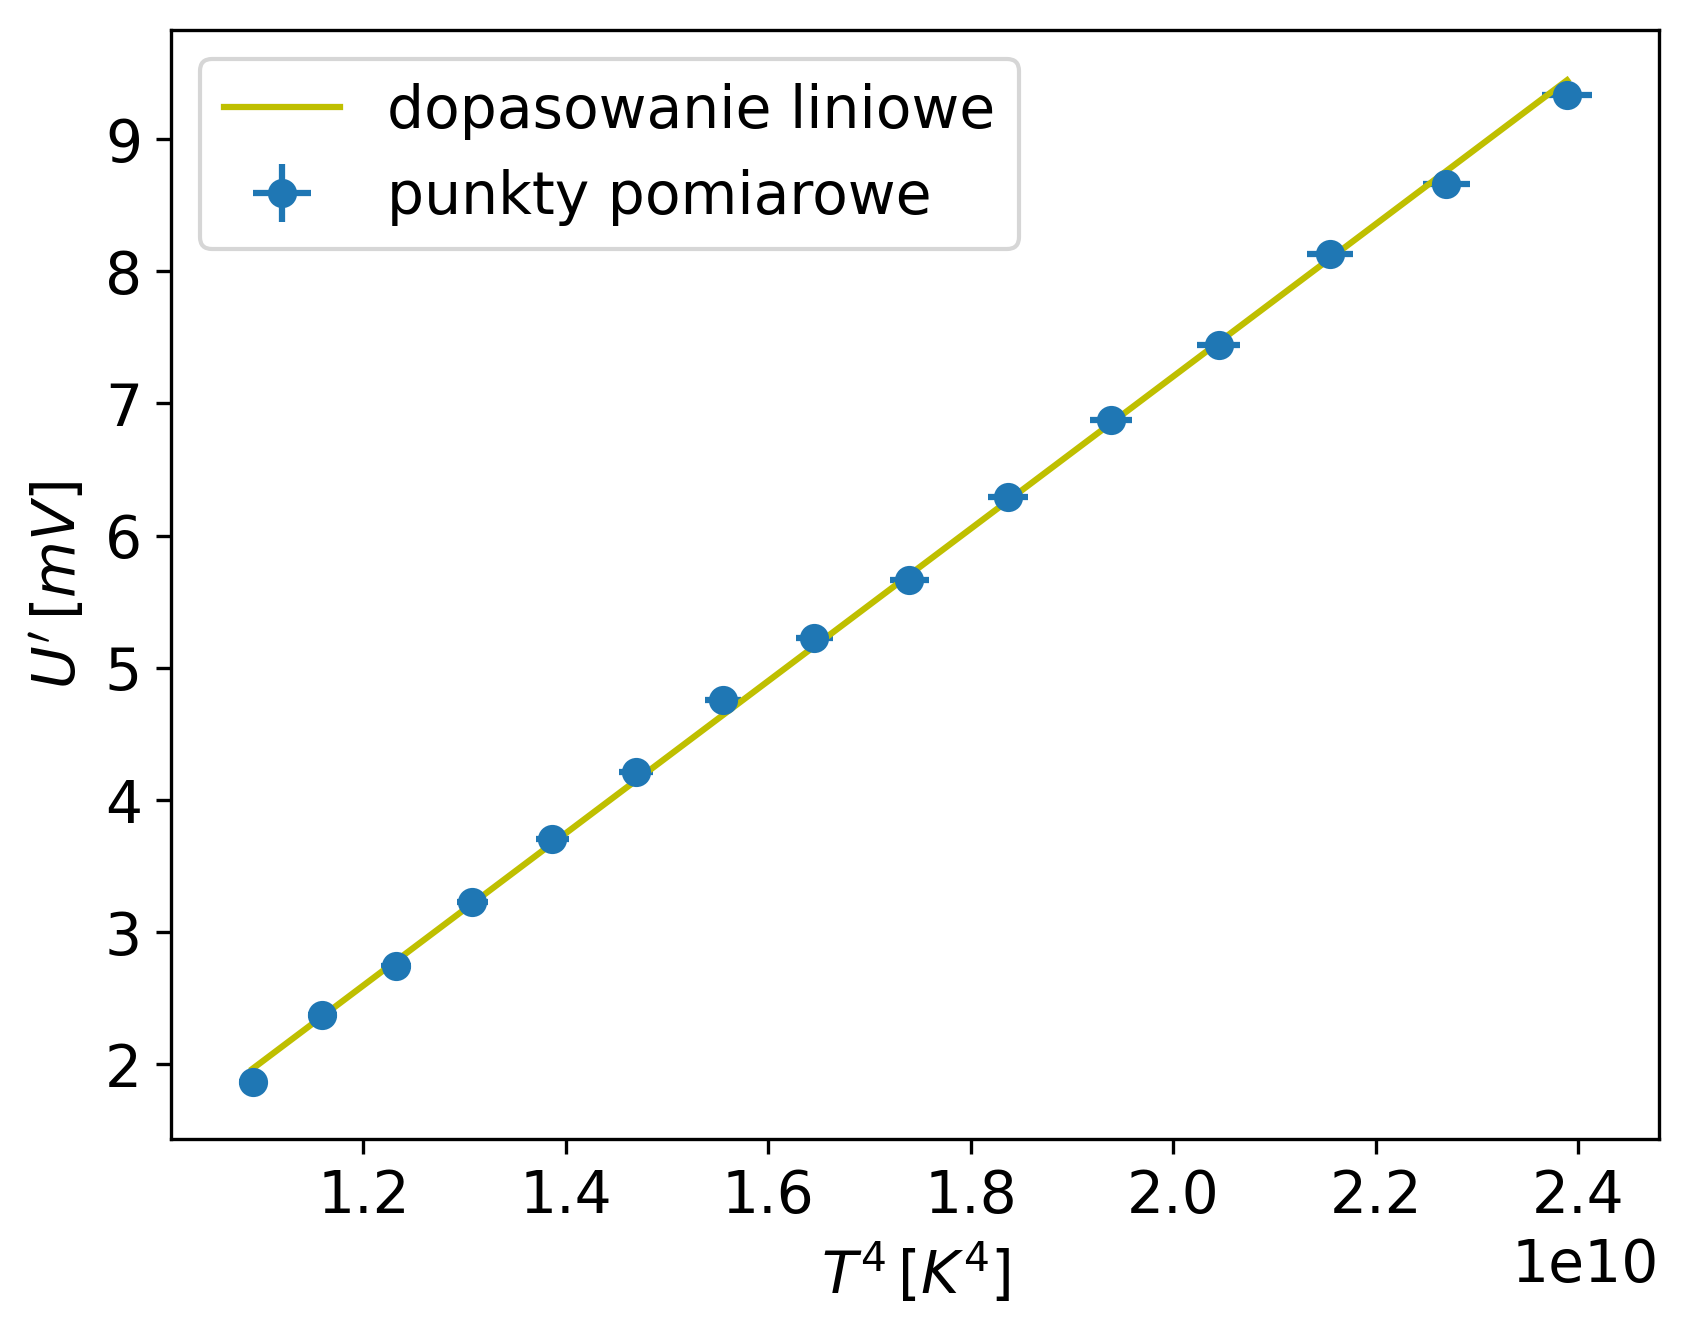
\includegraphics[width=\linewidth]{cube_white}
        \caption{biała}
        \label{fig:cube_white}
    \end{subfigure}
    
    \vspace{1em}

    \begin{subfigure}{0.45\textwidth}
        \centering
        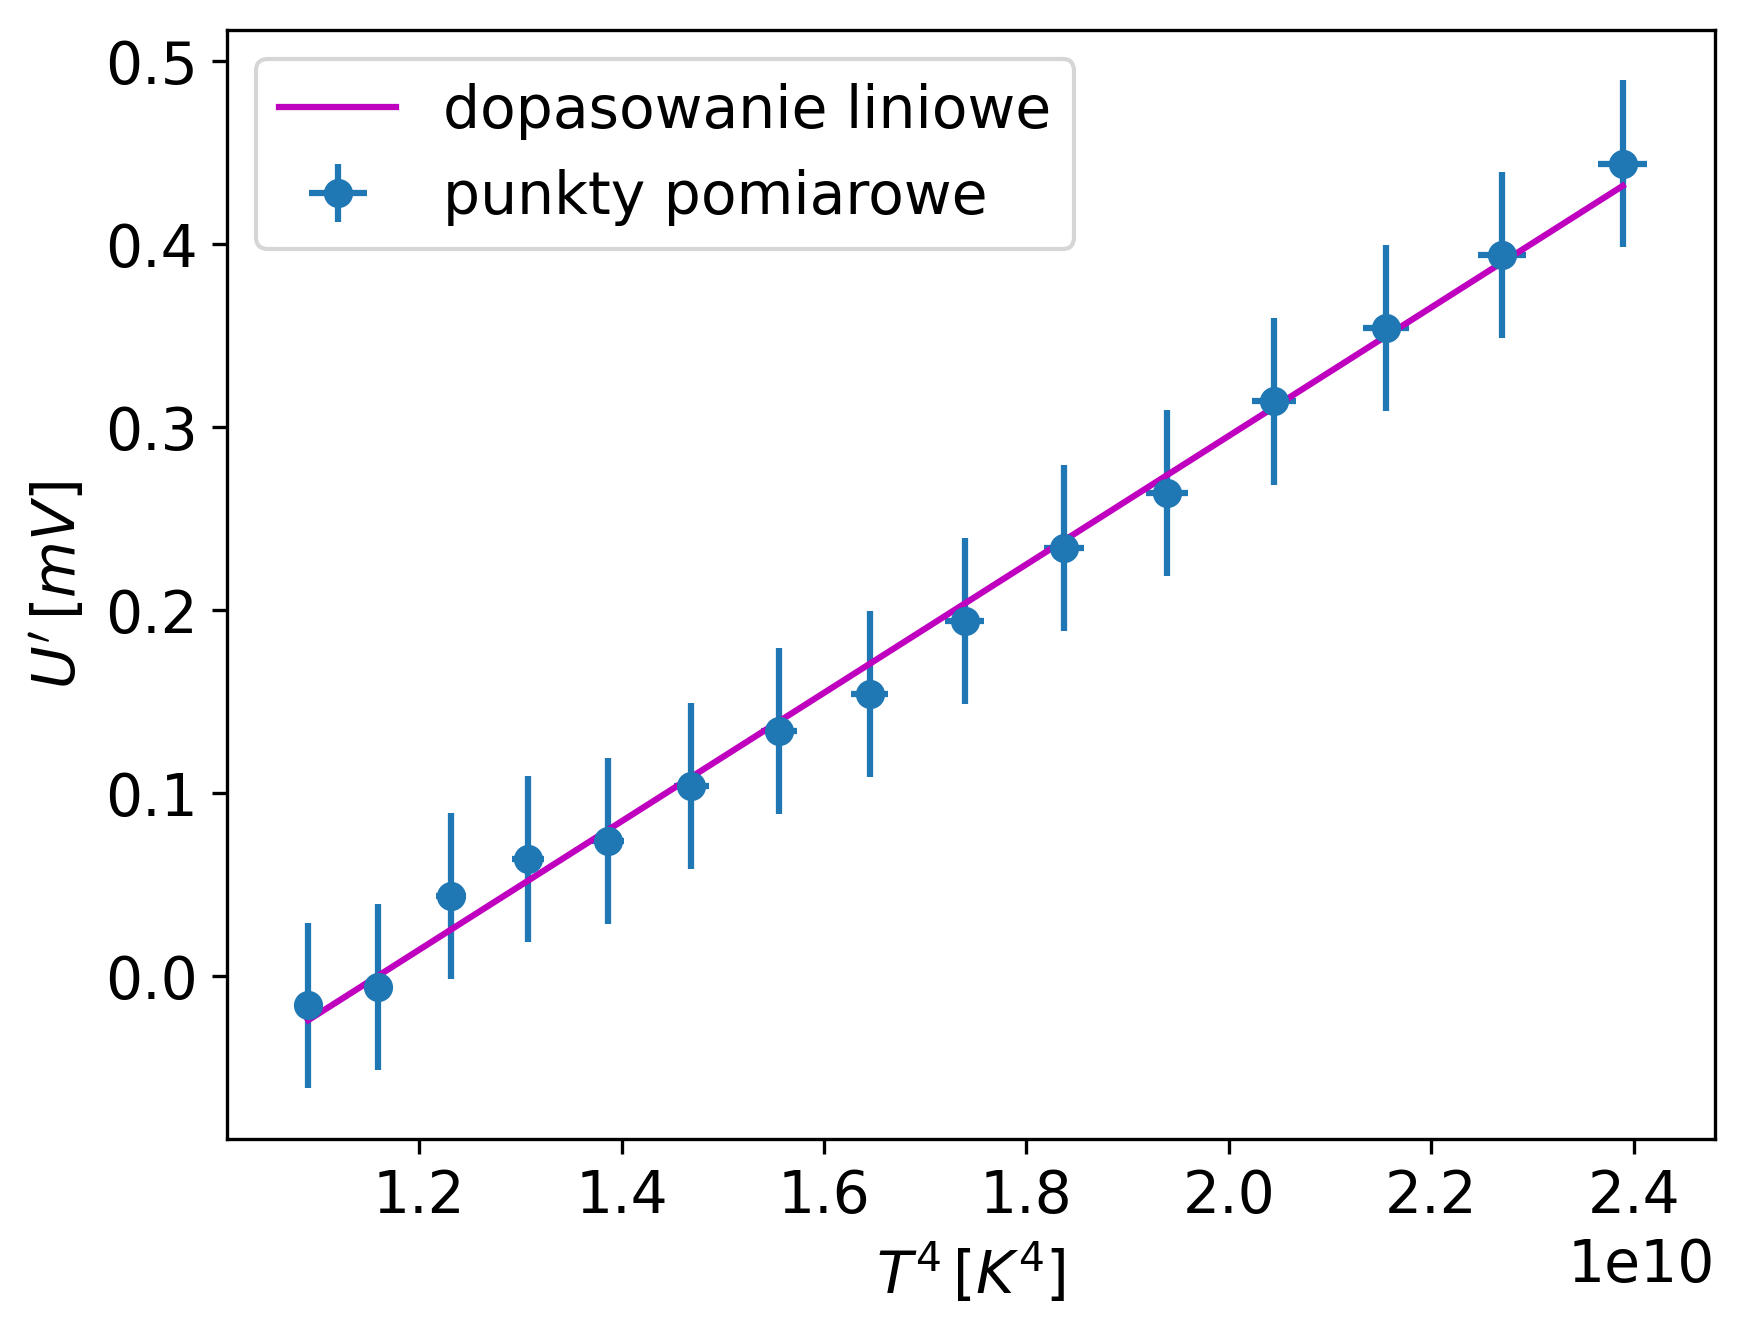
\includegraphics[width=\linewidth]{cube_shining}
        \caption{metalowa błyszcząca}
        \label{fig:cube_shining}
    \end{subfigure}
    \hfill
    \begin{subfigure}{0.45\textwidth}
        \centering
        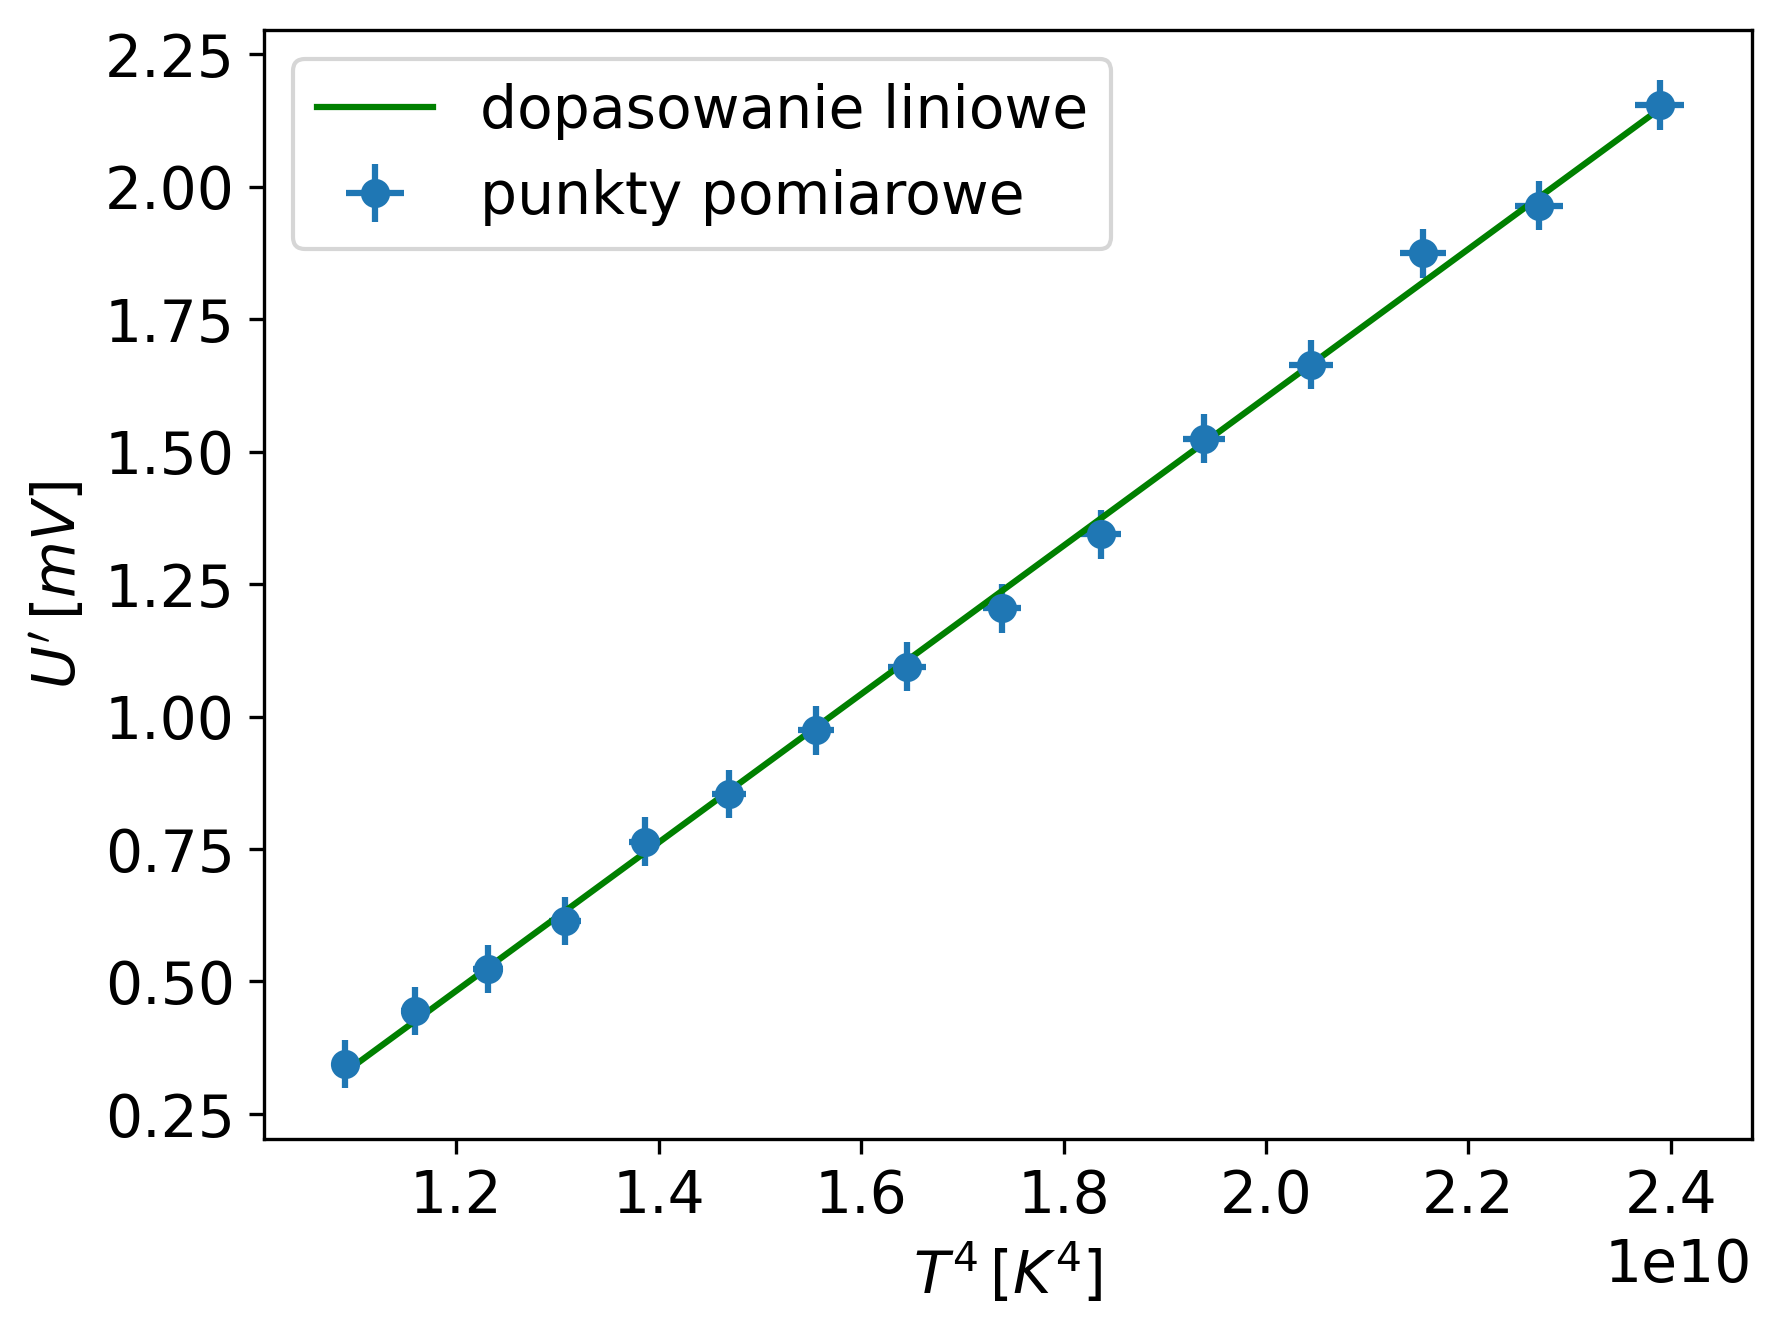
\includegraphics[width=\linewidth]{cube_dull}
        \caption{metalowa matowa}
        \label{fig:cube_dull}
    \end{subfigure}
    
    \caption{Wykres napięcia na detektorze $U'$ od temperatury kostki $T^4$ dla różnych ścian kostki Lesliego}
    \label{fig:cube_temp}
\end{figure}

Przyczyna błędu otrzymanego w dopasowaniach dla wykresów \ref{fig:cube_temp} zależy od materiału. Wszystkie powierzchnie posiadają te samę błędy dla temperatur i w przypadku powierzchni czarnej i białej to jest główny błąd jaki widzimy.
Natomiast gdy przejdziemy do ścian metalowych których promieniowanie powodowało znacznie mniejsze napięcie na detektorze, błąd pochodzący z tego pomiaru zaczyna mieć większy wpływ. Szczególnie jest to widoczne na wykresie \ref{} dla ściany metalowej błyszczącej.
Trzeba wspomnieć też o przyczynach niektórych błędów. Napięcie otoczenia mierzyliśmy podczas zasłonięcia kostki osłoną, lecz jak jest to widoczne w tabeli \ref{tab:cube_measurements} napięcie to znacznie się stosunkowo zwiększyło, najprawdopodobniej przez nagrzanie osłony.
Podobnie istnieje ryzyko że zapisaliśmy wartość napięcia za szybko. Starając się nie nagrzać detektora otkrywaliśmy go jak najkrócej lecz tak by napięcie mogło się ustabilizować, jednak w przypadku dużych temperatur trudno jest stwierdzić kiedy napięcie się ustabilizowałą a kiedy rośnie z powodu nagrzania detektora.

Otrzymane na wykresach \ref{fig:cube_temp} współczynniki kierunkowe zapisujemy w tabeli \ref{tab:cube_line}.
\begin{table}[H]
    \centering
    \begin{tabular}{c|cc}
        \toprule
        materiał ściany & $a [pVK^4]$ & $u(a) [pVK^4]$ \\
        \midrule
        czarna & 0{,}578 & 0{,}006 \\
        biała & 0{,}576 & 0{,}005 \\
        metal błyszczący  & 0{,}0351 & 0{,}0007 \\
        metal matowy & 0{,}1400 & 0{,}0015 \\
        \bottomrule
    \end{tabular}
    \caption{Współczynniki kierunkowe krzywych z \ref{fig:cube_temp}}
    \label{tab:cube_line}
\end{table}

Jako że w trakcie wszystkich pomiarów trzymaliśmy detektor nieruchomo oraz jego zależność napięcia od promieniowania jest liniowa \eqref{eq:measurment_device} możemy wyznaczyć emisyjność w prawie Stefana-Boltzmana \eqref{eq:boltzman_law_epsilon} znając emisyjność jednej ze stron i porównując ich dopasowanie (tab. \ref{tab:cube_line}.
Zatem załóżmy że strona czarna posiada $\epsilon_b = 0{,}95$ przy innych parametrach identycznych dla każdej ściany. Użyjemy wzór:
\begin{equation}
    \epsilon_o = \epsilon_b \frac{a_o}{a_b} \quad u(\epsilon_o) = \epsilon_o \sqrt{(\frac{u(a_o)}{a_o})^2 + (\frac{u(a_b)}{a_b})^2}
    \label{eq:epsilon_ratio}
\end{equation}
We wzorze $\epsilon_o$ jest emisyjnością innego materiału, a stałe $a_b$ i $a_o$ to współczynniki kierunkowe dla krzywej jakie otrzymaliśmy z dopasowania liniowego. Do otrzymania $u(\epsilon_o)$ wykorzystaliśmy wzór na propagecję błędu \eqref{eq:error_propagation}.
Podstawiając wartości z \ref{tab:cube_line} do \eqref{eq:epsilon_ratio} otrzymane wartości otrzymujemy:

\begin{table}[H]
    \centering
    \begin{tabular}{c|cc}
        \toprule
        materiał ściany & $\epsilon$ & $u(\epsilon)$ \\
        \midrule
        biała & 0{,}946 & 0{,}011 \\
        metal błyszczący  & 0{,}0576 & 0{,}0012 \\
        metal matowy & 0{,}230 & 0{,}003 \\
        \bottomrule
    \end{tabular}
    \caption{Wyznaczone za pomocą danych tabeli \ref{tab:cube_measurements} emisyjności $\epsilon$ i ich błędu $u(\epsilon)$ przy założeniu że czarna ściana posiada emisyjność $\epsilon = 0{,}95$.}
    \label{tab:materials_emisity}
\end{table}


\subsection{Żarówka Boltzmana}

Wpierw zbadajmy zależność odbieranego przez detektor promieniowania od temperatury włókna żarówki w przypadku stałej odległości $r = 5 \, cm$.
\begin{table}[H]
    \centering
    \begin{tabular}{c|cc|c|c|cc}
        \toprule
        Nr & $U_{l}$ [V] & $I_{l}$ [A] & $U_{d}$ [mV] & $U_{s}$ [mV] & $T$ [K] & $\delta T$ [K] \\
        \midrule
        1  & 0{,}828 & 0{,}919 & 0{,}15 & 0{,}05 & 781{,}69 & 18{,}81 \\
        2  & 1{,}775 & 1{,}191 & 1{,}13 & 0{,}05 & 1182{,}75 & 27{,}41 \\
        3  & 2{,}725 & 1{,}432 & 2{,}89 & 0{,}05 & 1449{,}35 & 32{,}87 \\
        4  & 3{,}681 & 1{,}648 & 5{,}68 & 0{,}07 & 1657{,}25 & 37{,}06 \\
        5  & 4{,}64  & 1{,}847 & 9{,}12 & 0{,}08 & 1829{,}17 & 44{,}02 \\
        6  & 5{,}60  & 2{,}033 & 12{,}31 & 0{,}06 & 1976{,}70 & 46{,}42 \\
        7  & 6{,}57  & 2{,}207 & 16{,}15 & 0{,}09 & 2110{,}54 & 48{,}71 \\
        8  & 7{,}53  & 2{,}370 & 20{,}25 & 0{,}08 & 2230{,}01 & 50{,}81 \\
        9  & 8{,}50  & 2{,}524 & 25{,}13 & 0{,}10 & 2342{,}70 & 52{,}84 \\
        10 & 9{,}47  & 2{,}671 & 30{,}24 & 0{,}11 & 2447{,}17 & 54{,}76 \\
        \bottomrule
    \end{tabular}
    \caption{Pomiar napięcia $U_d$ na detektorze dla różnych napięć $U_l$ i natężeń $I_l$ na żarówce bez zasłon i $U_s$ z zasłoną wraz z temperaturą na żarówce otrzymaną ze wzoru \eqref{eq:temp_bulb}.}
    \label{tab:temp_measurements}
\end{table}

Z otrzymanych danych oraz wzoru dla detektora \eqref{eq:measurment_device}, jesteśmy w stanie przeprowadzić walidację prawa Stefana-Boltzmana \eqref{eq:boltzman_law}, poprzez dopasowanie krzywej zależności $U' = U_d - U_s$ od $T^4$ do danych \ref{tab:temp_measurements} i zastosowanie testu $\chi^2$.
Jak w przypadku kostki zaczynamy od średniej z promieniowania pokoju.
\[
    \bar{U_s} = 0{,}074 \, [mV], \quad s_{U_s} = 0{,}021 \, [mV], \quad U_s = 0{,}020 \, [mV], \quad U_s = 0{,}024 \, [mV]
\]

\begin{figure}[H]
    \centering
    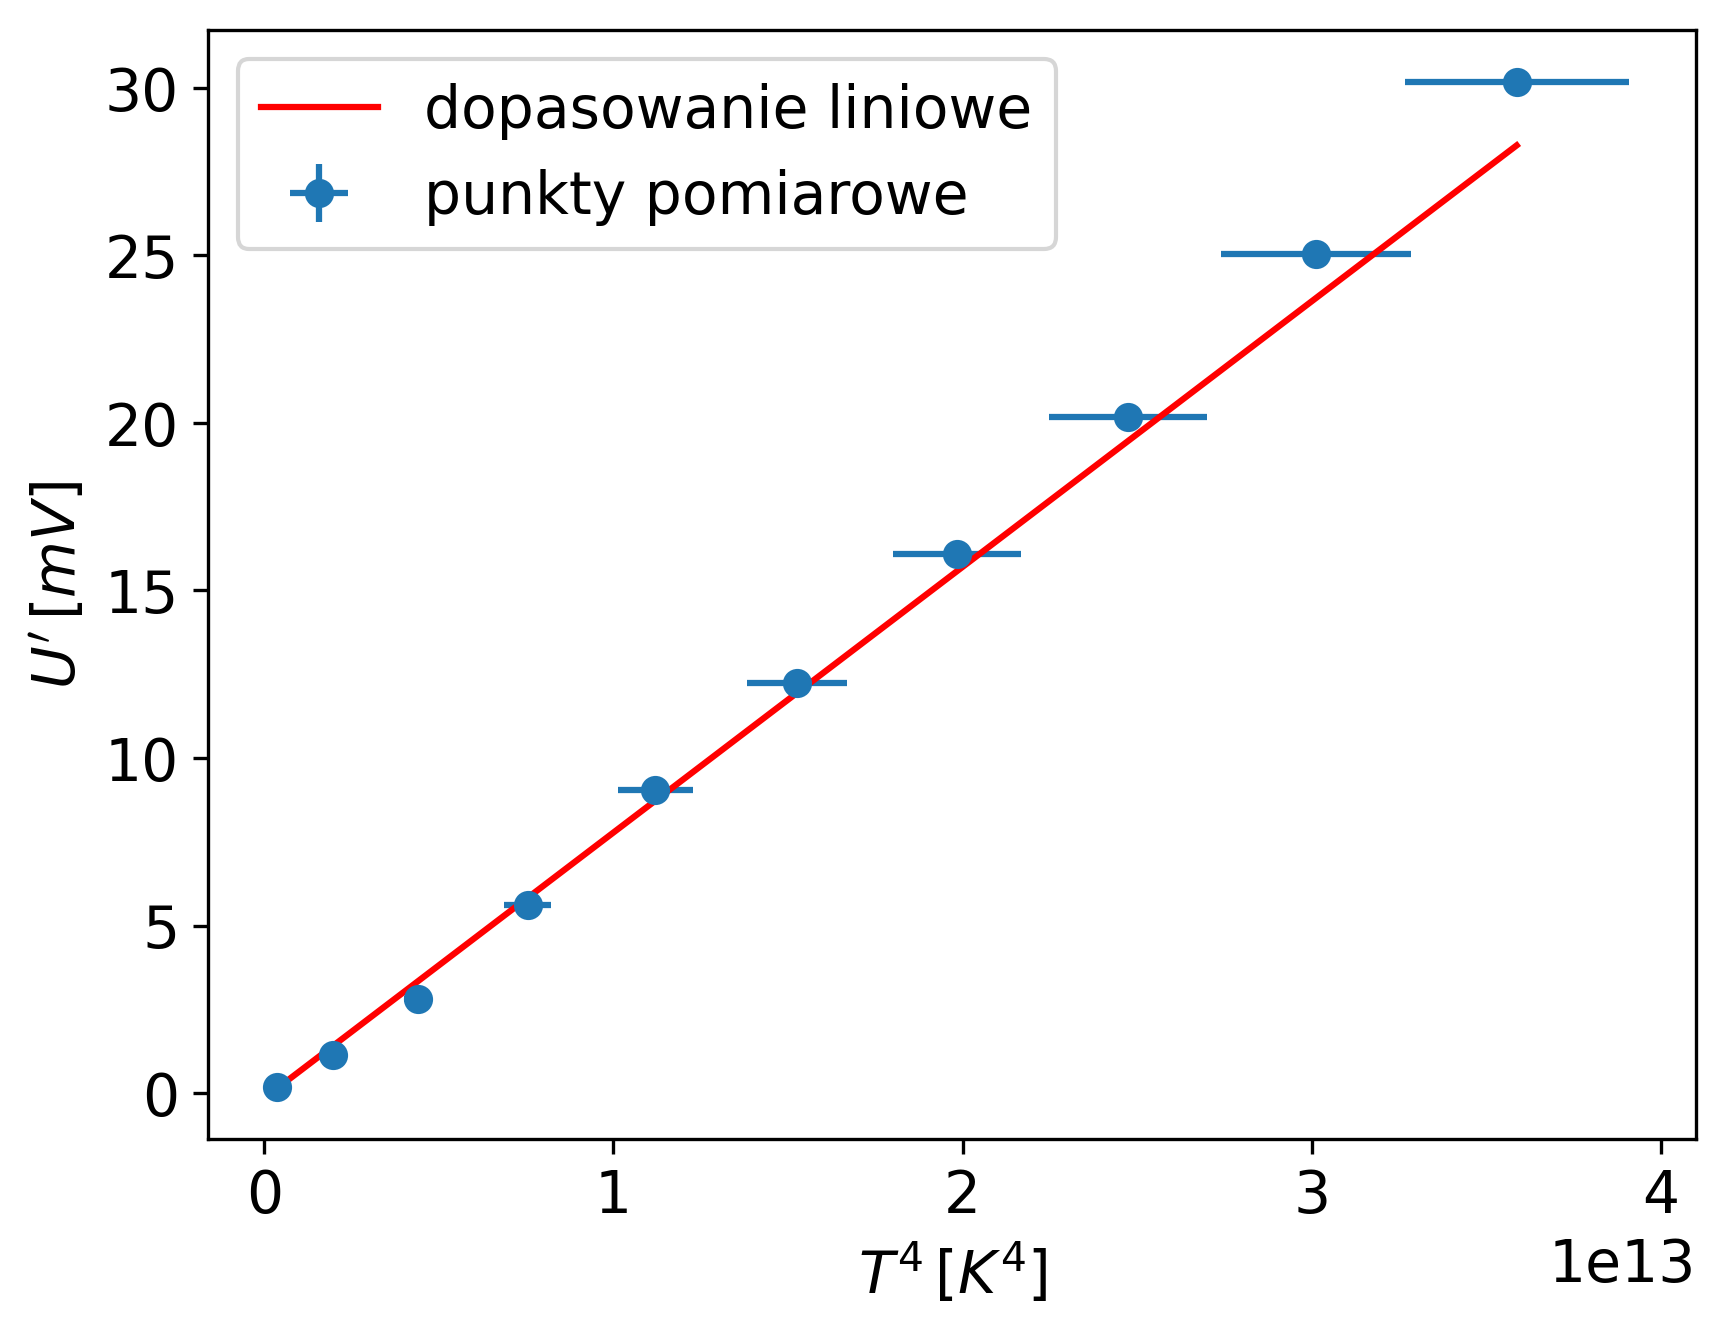
\includegraphics[scale=0.5]{boltzman_temp}
    \caption{Zależność zredukowanego napięcia na detektorze $U'$ od temperatury w czwartej potędze $T^4$ dla żarówki boltzmana o zmiennej temperaturze i stałej odległości.}
    \label{fig:boltzman_temp}
\end{figure}

Dla równania lini $U' = a_{l_t} T^4 + b_{l_t}$ trzymaliśmy parametry lini:
\[
    a_{l_t} = 0{,}79 \, [fVK^4], \quad u(a_{l_t}) = 0{,}03 \, [fVK^4]
\]
\[
    b_{l_t} = -0{,}15 \, [mV], \quad u(b_{l_t}) = 0{,}05 \, [mV]
\]
Do testu $\chi^2$ wykorzystamy powyżej wyznaczone parametry podstawione do wzoru~\eqref{eq:chi2} do którego podstawiamy zależność liniową:
\[
    \chi^2 = 8{,}36 
\]
Przy stopniach swobody $df = 10 - 2 =8$ test pokazuje że oszacowanie liniowe dokładnie opisuje dane. Spowodowane jest to dużym błędem dla większych temperatur $\delta (T^4) = 4T^3 \, \delta T$ widocznym na rys.~\ref{fig:boltzman_temp}.

Następnie przebadajmy zależność promieniowania od odległości źródła dla pomiarów ze stałym napięciem $U_l = 9{,}47$ i natężeniem $I_l = 2{,}670$ na żarówce.
\begin{table}[H]
    \centering
    \begin{tabular}{c|c|c|c}
        \toprule
        Nr & $d$ [cm] & $U_d$ [mV] & $U_s$ [mV] \\
        \midrule
        1 & 149 & 30{,}58 & 0{,}12 \\
        2 & 144 & 9{,}29  & 0{,}10 \\
        3 & 139 & 4{,}11  & 0{,}11 \\
        4 & 134 & 2{,}36  & 0{,}11 \\
        5 & 129 & 1{,}52  & 0{,}11 \\
        6 & 124 & 1{,}08  & 0{,}08 \\
        7 & 119 & 0{,}82  & 0{,}06 \\
        8 & 114 & 0{,}64  & 0{,}05 \\
        9 & 109 & 0{,}52  & 0{,}05 \\
        \bottomrule
    \end{tabular}
    \caption{Pomiar napięcia $U_d$ na detektorze dla różnych znaczników na szynie $d$, oraz pomiar napięcia powodowany przez tło $U_s$.}
    \label{tab:distance_measurements}
\end{table}
W tabeli \ref{tab:distance_measurements} $d$ oznacza dystans jaki odczytaliśmy na szynie w momęcie gdy żarówka znajdowała się na $d_0 = 154 \, cm$.
Dla obu pomiarów dystansów $d$ oraz $d_0$ zakładamy że błąd wynosi $\delta d = 0{,}5 \, mm$ czyli połowe podziałki.
Na podstawie wzorów \eqref{eq:power_flux} oras \eqref{eq:measurment_device} zakładamy że napięcie będzie proporcjonalne do $\frac{1}{r^2}$. 
W celu przetestowania tej hipotezy dopasujmy krzywą do zależności $\log(U')$ od $\log(r)$ gdzie $r = |d-d_0|$ a $U' = U_d - \bar{U_s}$.

\begin{figure}[H]
    \centering
    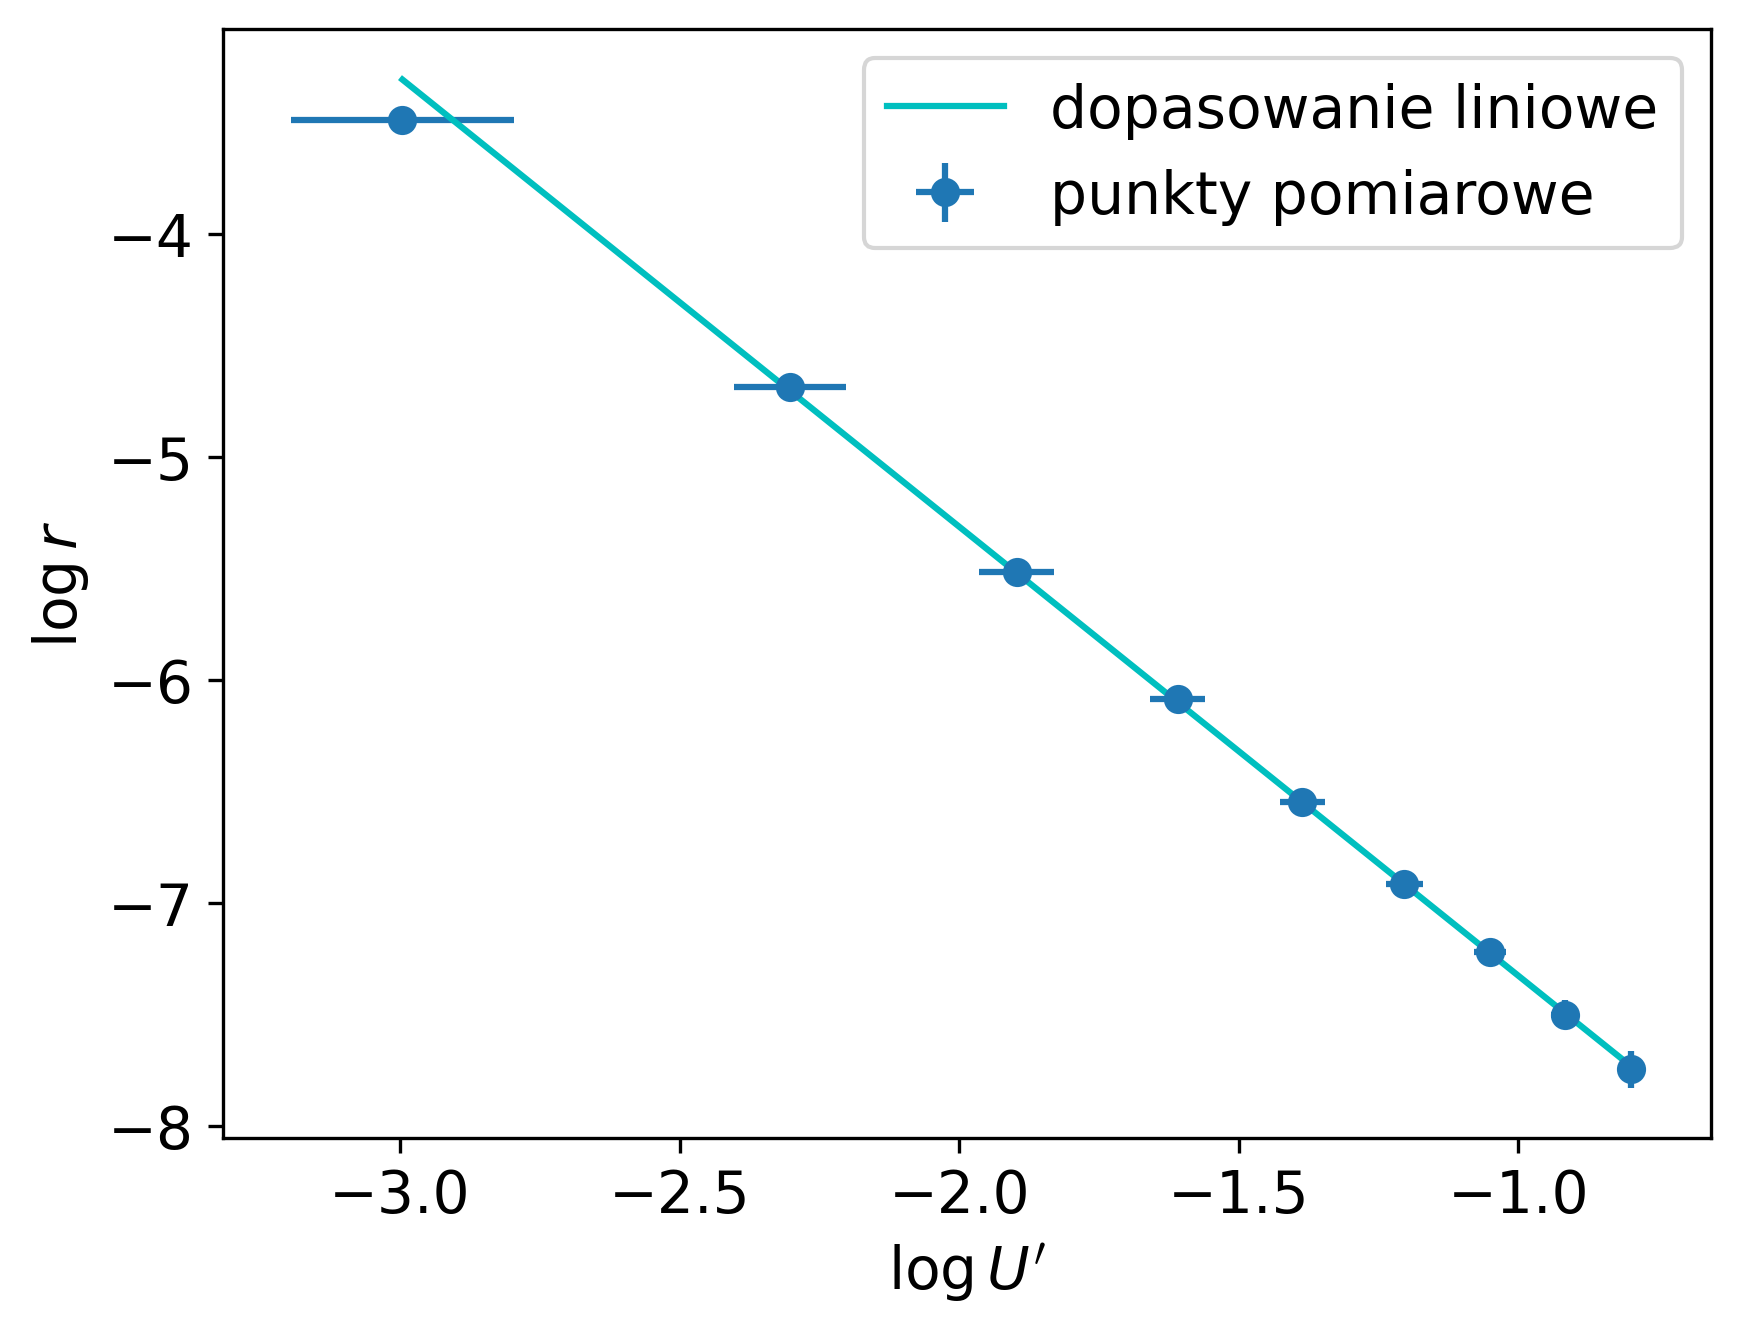
\includegraphics[scale=0.5]{boltzman_distance}
    \caption{Zależność logarytmu zredukowanego napięcia na detektorze $\log{U'}$ od logarytmu z odległości między detektorem a źródłem $\log{r}$ dla żarówki boltzmana o stałej temperaturze.}
    \label{fig:boltzman_distance}
\end{figure}

Dopasowane parametry do lini $\log(U') = a_{l_d} \log(r) + b_{l_d}$ widniejącej na rys.~\ref{fig:boltzman_distance} wynoszą
\[
    a_{l_d} = -2{,}013 \quad u(a_{l_d}) = 0{,}017
\]
\[
    b_{l_d} = -9{,}34, \quad u(b_{l_d}) = 0{,}03
\]
Podobnie jak w przypadku zależności temperaturowej wykorzystujemy test $\chi^2$~\eqref{eq:chi2}:
\[
    \chi^2 = 0{,}97
\]
W tym przypadku nasze stopnie swobody wynoszą $df = 9 - 2 = 7$, a test pokazuje że dane bardzo dokładnie są opisywane przez zależność $U' = cr^{-2}$ co przez wzór \eqref{eq:measurment_device} przekłada się na zależność opisywaną we wzorze \eqref{eq:power_flux}.

\subsection{Transmisyjność Szkła}
Możemy również wyciągnąć pewne wnioski o transmisyjności szkła z dwóch pomiarów jakie wykonaliśmy. Najpierw porównajmy pomiar detektora dla czarnej ściany kostki Lesliego w temperaturze $T = 150 \, ^{\circ}C$ (tab. \ref{tab:cube_glass}. Później wyznaczmy wartości napięcia na detektorze dla żarówki oddalonej o $r = 5 \, cm$ od detektora, na której jest napięcie $U = 9{,}47 \, V$ i przepływa natężenie $I = 2{,}670 \, A$ (tab. \ref{tab:bulb_glass}.
\begin{table}[H]
    \centering
    \begin{tabular}{cc}
        \toprule
        Pomiar & $U_d$ \\
        \midrule
        Bez szkła & 9{,}53 \\
        Szkło & 0{,}19 \\
        \bottomrule
    \end{tabular}
    \caption{Porównanie pomiarów napięcia na detektorze promieniowania od kostki Lesliego z ekranem szklanym pomiędzy kostką i detektorem oraz bez.}
    \label{tab:cube_glass}
\end{table}
\begin{table}[H]
    \centering
    \begin{tabular}{cc}
        \toprule
        Pomiar & $U_d$ \\
        \midrule
        Bez szkła & 30{,}24 \\
        Szkło & 22{,}10 \\
        \bottomrule
    \end{tabular}
    \caption{Porównanie pomiarów napięcia na detektorze promieniowania od żarówki z ekranem szklanym pomiędzy żarówką i detektorem oraz bez.}
    \label{tab:bulb_glass}
\end{table}
Jesteśmy w stanie zauważyć że w przypadku czarnej ściany kostki (tab. \ref{tab:cube_glass}) szkoło blokuje praktycznie całe promieniowanie, odbierane przez nas prowmieniowanie było na poziomie tego obieranego z reszty pokoju podczas innych pomiarów. Natomiast gdy proównujemy napięcie powodowane przez promieniowanie wywoływane przez żarówkę za szybą i bez (tab. \ref{tab:bulb_glass} widzimy spadek jednak ani trochę tak spektakularnego jak w przypadku kostki (tab. \ref{tab:cube_glass}).

\begin{figure}[H]
    \centering
    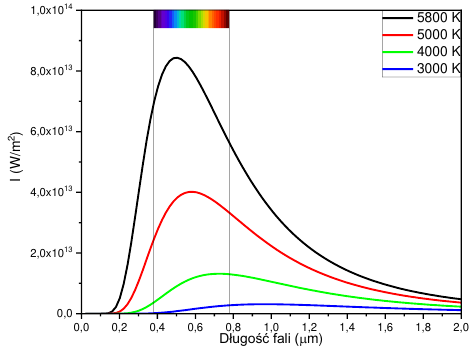
\includegraphics[scale=0.65]{black_body}
    \caption{Wykres zależności \eqref{eq:emision_spectrum} pochodzący z \cite{skrypt}}
    \label{fig:black_body}
\end{figure}

Z tych pomoarów oraz wykresu~\ref{fig:black_body} możemy wywnioskować że transmisyjność szkła dla promieni podczerwonych które dominowały w pomiarach dla kostki jest bliska zera, dlatego widzimy taki spadek napięcia w tabel \ref{tab:cube_glass}. Podczas gdy transmisyjność szkoła w przypadku światła widzialnego jest wysoka. Mimo to wciąż widzimy spadek w  przypadku żarówki (stosunek napięcia bez szkła do tego ze szkłem wynosi $73\%$), najpewniej spowodowane obecnością część energi w promieniowaniu podczerwonym i innych spektrach dla których szkło nie ma $100\%$ transmisyjności.

\section{Podsumowanie}



\newpage

\begin{thebibliography}{3}

\bibitem{skrypt}
\emph{Badanie Promieniowaniia Termicznego}, Uniwersytet Warszawski, Aneta Drabińska.

\bibitem{radiation_multimeter}
\url{brymen.eu/wp-content/uploads/biall/102091/102091.KARTA_EN..2015-07-08.1.pdf}, miernik uniwersalny BRYMEN BM827s.

\bibitem{bulb_multimeter}
\url{https://static.eleshop.nl/mage/media/downloads/bm805_datasheet.pdf}, miernik uniwersalny BRYMEN BM 805s.
\end{thebibliography}

\end{document}
